\chapter{Web Technologies}
\label{chapter:WebTechnologies} 

In this chapter, we will introduce the basic elements for communication in the Internet. We will start with Internet-based communication protocols, then move onto web communication protocols. Furthermore, we will compare traditional communication technology with modern HTML5 communication technologies. Among the HTML5 communication technologies, we focus on the WebSocket protocol and its relevant subprotocols.

\section{Internet-based Communication Protocols}

\subsection{TCP, UDP and IP}
Transmission Control Protocol (TCP), one of the two major transport-layer protocols, provides a reliable bi-directional communication \cite{comer2008computer}. TCP addresses the communication problem between applications with the following major features: 

\begin{itemize}
% You can use this command to set the items in the list closer to each other
% (ITEM SEParation, the vertical space between the list items) 
\setlength{\itemsep}{0pt}
\item Transferring Data over a connection;
\item Connecting two endpoints;
\item Data is received the same as it is delivered;
\item Data is sent in sequence;
\item Reliable startup and shutdown;
\end{itemize}

The User Datagram Protocol (UDP) is the other major transport-layer protocol used in the Internet \cite{comer2008computer}. Compared with TCP, UDP is less complex and thus less reliable. For example, UDP is connectionless, meaning a message can be sent between two endpoints without prior arrangement; UDP sends and receives individual messages, meaning it does not divide a message into multiple parts.

The Internet Protocol (IP) provides a communication mechanism for computers or devices \cite{postel1981internet}. IP distinguishes each computer or device in network by a unique number known as Internet Protocol Address (IP address). TCP or UDP packets are usually encapsulated into IP packets.

\subsection{HTTP}

Hypertext Transfer Protocol (HTTP) is an application layer protocol exchanging or transferring contents, such as hypertext, in request/response pattern \cite{fielding1999hypertext}. HTTP is assigned to port number 80 over either TCP or UDP connection \cite{reynolds1994assigned}. HTTP communication, however, usually is established over TCP/IP connections with the default port TCP 80. HTTP can be also established other protocol, such as unreliable UDP.

When a browser requests resources from a server, usually the browser sends a HTTP request to the server. Then the server answers with an HTTP response. Before HTTP 1.1, a pair of request/response is, usually, sent in a single TCP connection. Generally, a TCP connection is expensive to create, while most HTTP 1.0 or older connections use TCP at least efficiency, which leads to congestion and unwanted overhead \cite{spero1994analysis}.  To improve this, HTTP provides connection reuse mechanism \cite{fieldingrfc} by using Keep-Alive in general headers. This mechanism has been further improved in HTTP 1.1, and thus all connections are set to persistency by default. This mechanism aims for reducing CPU and memory usage, pipelining, reducing network congestion, reducing latency the frequency of TCP opening handshakes and error reported improvement. With pipelining, the performance of HTTP 1.1 can be largely improved compared with HTTP 1.0 \cite{nielsen1997network}. 

At this point, HTTP persistent connections seem to be perfect and the WebSocket protocol is unnecessary. The HTTP persistent connection, however, is restricted by its practical consideration. Firstly, Servers are, usually, maintained by setting time-out value. Consequently, the mechanism kills idle connections. e.g. Apache 2.0 server will set the timeout at 15 seconds by default\footnote{http://httpd.apache.org/docs/2.0/mod/core.html\#keepalivetimeout}, while Apache 2.2 reduces the amount down to 5 seconds\footnote{http://httpd.apache.org/docs/2.2/mod/core.html\#keepalivetimeout}. Additionally, this implies that both clients and servers need to be capable to recover from any closed events and subsequently indicates delay in communication. Secondly, any client that use persistent connections is instructed to limit the number of simultaneous connections that they maintain to a given server at the maximum of two, for the purpose of improving HTTP response time and avoiding congestion. 

For a browser, in order to synchronise the information with a web server, normally, there are polling or long-polling over Ajax. When we use Ajax, we retrieve data from a remote server by sending an HTTP Request; and if we would like to retrieve more data, we need to send other HTTP Requests. HTTP request/response will, finally, confront with the fact that it increases the frequency of requesting the web server, with repeatedly connections and disconnections; or increases the workload of the web server to keep the requests open. The problem becomes severe when it happens in the scenario of Internet of Things (IoT) with a large amount of devices interconnected. Figure \ref{fig:client-server-http} illustrates sequence diagram where a client (browser) fetches data from a server using HTTP.

\begin{figure}[t]
  \begin{center}
    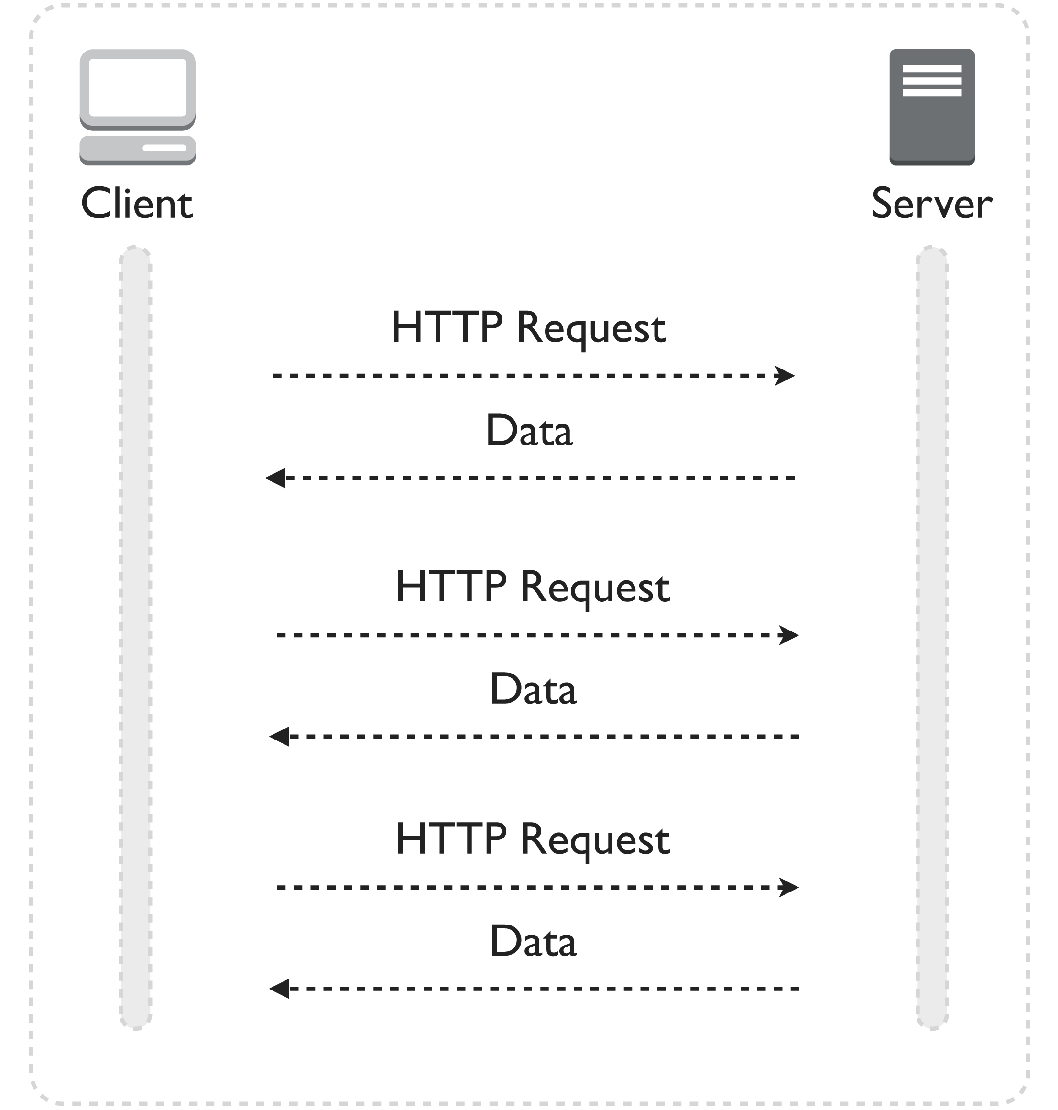
\includegraphics[width=0.5\textwidth]{images/client-server-http.pdf}
    \caption{A Client Fetches Data from A Server with HTTP}
    \label{fig:client-server-http}
  \end{center}
\end{figure}

\subsection{HTML5}
\label{HTML5}

HTML5 is hypernym that consist of a large number of web technology \cite{wang2012definitive}. HTML5 covers the following area: new semantics, new CSS styling, multimedia, Graphics and 3D, Device Access, Performance, offline \& storage and connectivity. Amount all, the connectivity consists of communication technology such as Web Real-Time Communications (WebRTC), Server-Sent Events (SSE), Cross-Document messaging and WebSocket. WebRTC\footnote{http://www.webrtc.org/reference/architecture} provides realtime multimedia communication on web without requiring plugins; SSE provides an API for a browser to receive pushing notification from a server via an HTTP connection \cite{hickson2009server}; While Cross-Document messaging or Web Messaging largely expands the possibility and capability of communication of web browsers with least side-effect on security and privacy. Cross-Document messaging is designed to overcome the same-origin policy.

The WebSocket Protocol is also a part of HTML5 and will be discussed in Subsection \ref{websocket}.

\section{Traditional Communication}

The client/server model is one of the network architectures to connect computers or applications, where the server provides resources and the client requests for the resources. Usually, the client/server model is designed as a request/response model, where the server does not actively communicate with clients. The client could be a computer, or an application, such as a web browser. The server is, usually, a (powerful) computer that keeps some applications running as constantly as possible. Those applications could be a database, a web server (application), or a printer server (application) that links to a physical printer. 

The HTTP protocol is a request/response protocol \cite{fielding1999hypertext}, where a client, or rather a user agent (UA) communicates with a server through a request and a response message(s). In other words, a client retrieves resources from a server in a request message, while the server hands over the contents in a response message. This is a general model that a client retrieves data from a server. A classic web page must reload, when a web browser updates the content, whose procedure generates a large amount of additional overheads. With Ajax, a technique allowing web pages to be updated asynchronously, web pages can be updated partially as needed, without reloading the whole page. This procedure exchanges less amount of data compared with the classic web pages updating. 

Generally, there are three ways to retrieve data asynchronously\cite{lubbers2010html5}: polling, long polling and streaming. All these approaches are uni-directional. 

With \emph{polling}, a client sends a request to a server, e.g. a web browser sends a request with Asynchronous JavaScript and XML (Ajax) \cite{garrett2005ajax} to a web server and expects data. This is an efficient solution, if the client knows exactly the time when the data is available. However, the server might not have the content when the client requests, or the content may be temporarily unavailable. If this situation would happen in practise, the client would have repeated polling for data. This will result in a large redundant headers generated by HTTP protocol, and a hight number of TCP connections. Consequently, the approach leads a heavy workload to the server and will not be suitable in the scenario, such as, some Internet scenarios with a large number of nodes. 

Another method, Long polling, is an improved approach, with respect to the frequency of request. Compared with polling, long polling does similarly, expect that the server holds the client's request for a certain period until timeout. Within this period, the server will send a response(s) back to the client, if there is data available. This method reduces the frequency of HTTP requests, but it increases the workload of a server, such as, ports handling. Generally, an HTTP request is initiated over TCP/IP connections (but any other protocols that guarantee a reliable transport can be used) \cite {fielding1999hypertext}. In TCP/IP connections, a port number is 16 bits \cite{postel2003rfc}, which means the maximum number of ports is \(  2^{16}  = 65536 \). However, one characteristic in the aforementioned Internet scenarios is scalability, which means the number of nodes could yield to a larger amount than that of the ports. Even though all ports are dedicated to communication, it is insufficient to support the schema with a large number of Internet-based nodes. 

As for the HTTP streaming, or known as HTTP server push, a server sends a response and keeps the connection open and alive, where the connection is triggered by a client's request. The drawback of this approach is that streaming is still encapsulated in HTTP, and thus buffer mechanism might increase the latency of messages delivering. Moreover, buffer is not an approach for an energy constrained device.

\section{WebSocket}
\label{websocket}

The WebSocket Protocol enables full-duplex communication through a single socket between a client and a remote server. For this reason, this technology decreases the amount of opening ports on server sides, comparing with the traditional mean of retrieving resource. Moreover, this protocol is not just an enhancement of the current HTTP protocol; it, however, represents enormous advance, especially for real-time, event-driven communication \cite{lubbers2010html5}.

Moreover, the WebSocket protocol supports data frame including text and binary. Once the WebSocket connection has been successfully established, generally, data frames transfer between a client and a server. However, in consideration of optimising WebSocket connections between a client and a server, the client can request that the server use a specific subprotocol by including the |Sec-WebSocket-Protocol| filed in its handshakes \cite{rfc64552012web}. A subprotocol is a application-level protocols layered over the WebSocket protocol \cite{rfc64552012web}. A subprotocol could be implemented by the servers and can be also versioned. The server chooses one or none subprotocol. 

The goal of WebSocket technology is to provide a mechanism for browser-based applications that need two-way communication with servers that does not rely on opening multiple HTTP connections (e.g. using XMLHttpRequest or <iframe>s and long polling)\footnote{http://www.websocket.org}. Older web technology, like HTTP, remains inefficiencies problems \cite{wang2012definitive}. Firstly, it is not natively designed for nowadays Web Applications with rich contents and interactive demands; Secondly, overheads and unnecessary information cumulate swiftly as the interaction between the client and server continues. WebSocket improves communication problems by solving the above problems, while keeping simplicity. Both WebRTC and WebSocket are in effort to enhance the real-time communication. WebRTC provides APIs that allow web browsers communicate with each other directly, while WebSocket provides the real-time communication mechanism between a client and a server. Figure \ref{fig:client-server-ws} illustrates sequence diagram where a client (browser) fetches data from a server using WebSockets.

\begin{figure}[t]
  \begin{center}
    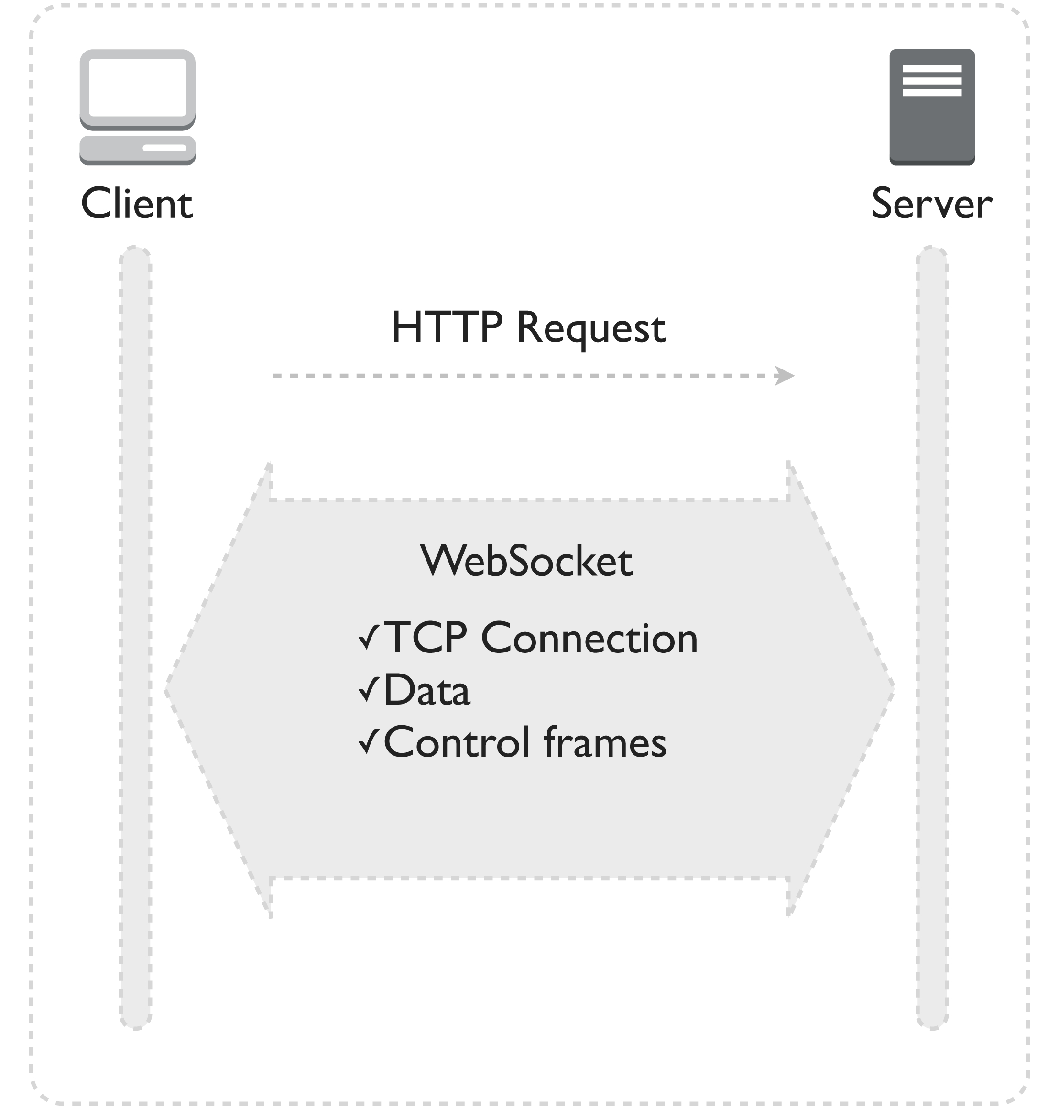
\includegraphics[width=0.5\textwidth]{images/client-server-ws.pdf}
    \caption{A Client Fetches Data from A Server with WebSockets}
    \label{fig:client-server-ws}
  \end{center}
\end{figure}

\subsection{WAMP}

WebSocket Application Messaging Protocol (WAMP)\footnote{http://wamp.ws/} is a subprotocol officially registered in WebSocket Protocol Registries\footnote{http://www.iana.org/assignments/websocket/websocket.xml\#subprotocol-name} , which gives structure to messaging by providing two hight level messaging patterns: Publish/Subscribe (Pub/Sub) and Remote Procedure Calls (RPC).

WAMP fills in the blanks in the WebSocket protocol: a low-level specification which originally provides raw messaging communication (text or binary). Moreover, WAMP does not make any extra standard, but it bases on established Web standards: WebSocket, JSON and URI. The WebSocket standard is the default transport channel where WAMP is binding. With the WebSocket Standard, WAMP is assumed to be given a reliable, ordered, and full-duplex message channel. 

\subsection{Other Registered Subprotocols}

Apart from WAMP, there are MessageBroker WebSocket Subprotocol (MBWS), Simple Object Access Protocol (SOAP) and Simple Text Oriented Messaging Protocol (STOMP) can be used as subprotocols, according to the WebSocket Protocol Registries.

MBWS is used by messaging clients to send messages to, and received messages from, an Internet message broker. The Internet message broker is also called a message broker which queues messages, sent by clients, for asynchronous deliveries to clients \cite{hapner2012messagebroker}. Like WAMP, MBWS provides full-duplex and reliable transport; unlike WAMP, MBWS does not obviously provide higher level messaging patterns. MBWS, however, defines a binary message frame starting with an MBWS binary header, and a text message frame starting with an MBWS text header. MBWS provides two additional features. Firstly, it supports connection recovery, which has not defined by the WebSocket protocol. Secondly, it supports metadata in MBWS message headers. MBWS has a light weight version, called MessageBrokerLight WebSocket Subprotocol (MBLWS) which only supports Message Metadata \cite{hapner2012messagebroker}. However, MBWS is still a draft. 

SOAP is a lightweight protocol intending for exchanging structured information in a decentralised and distributed environment. SOAP uses XML technology to exchange data \cite{gudginsoap}. Microsoft, additionally, defines SOAP Over WebSocket Protocol Binding (MS-SWSB)\footnote{http://msdn.microsoft.com/en-us/library/hh536812.aspx}, a subprotocol for the WebSocket Protocol. The subprotocol involves a Web Services Description Language (WSDL) and supports message exchange patterns (MEPs). With MEPs, SOAP supports one-way, two-way and request/response message exchange patterns, which involves Pub/Sub and RPC.

Simple (or Streaming) Text Orientated Messaging Protocol (STOMP)\footnote{http://stomp.github.io} is a frame-based protocol. It refers to a STOMP frame includes a command, optional headers and a body. STOMP is text-based with UTF-8 encoding by default, but it, optionally, supports binary messages. As for message patterns, STOMP version 1.2 supports Pub/Sub. An example of Pub/Sub model using STOMP with WebSocket is discussed in \cite{wang2012definitive}.

Table \ref{table:subprotocol-comparison} is a comparison summary among WAMP, MBWS, SOAP and STOMP:

% If you need to have linefeeds (\\) inside a cell, you must create a new
% paragraph-formatting environment inside the cell. Most common ones are 
% the minipage-environment and the \parbox command (see LaTeX documentation
% for details; or just google for ``LaTeX minipage'' and ``LaTeX parbox'').
\begin{table}
\begin{tabular}{|p{2.2cm}|>{\centering\arraybackslash}p{2.2cm}|>{\centering\arraybackslash}p{3cm}|>{\centering\arraybackslash}p{1.5cm}|>{\centering\arraybackslash}p{2.9cm}|} 
% Alignment of sells: l=left, c=center, r=right. 
% If you want wrapping lines, use p{width} exact cell widths.
% If you want vertical lines between columns, write | above between the letters
% Horizontal lines are generated with the \hline command:
\hline % The line on top of the table
\textbf{ } & \textbf{WAMP} & \textbf{MBWS} & \textbf{SOAP} & \textbf{STOMP} \\ 
\hline 
% Place a & between the columns
% In the end of the line, use two backslashes \\ to break the line,
% then place a \hline to make a horizontal line below the row 
\textbf{Data Representation} & JSON & binary and text with MBWS headers & XML & binary and text with headers \\ 
\hline
\textbf{Message Patten} & Pub/Sub, RPC & not specified & MEP & Pub/Sub \\
% The multicolumn command takes the following 3 arguments: 
% the number of cells to merge, the cell formatting for the new cell, and the
% contents of the cell
\hline
\textbf{Connection Recovery} & no & yes & no & no \\
\hline
\textbf{Metadata} & currently no & yes & yes & no \\
\hline
\textbf{Released} & yes & draft & yes & yes \\
\hline
\end{tabular} % for really simple tables, you can just use tabular
% You can place the caption either below (like here) or above the table
\caption{WAMP and other WebSocket subprotocols}
\label{table:subprotocol-comparison}
\end{table} % table makes a floating object with a title
